%----------------------------------------------------------------------------------------
% DOCUMENT CONFIGURATION
%----------------------------------------------------------------------------------------
\documentclass[10pt,english,french]{article}

%----------------------------------------------------------------------------------------
% ENCODING
%----------------------------------------------------------------------------------------
\usepackage[T1]{fontenc}
\usepackage[utf8]{inputenc}
\usepackage[USenglish, french]{isodate}
\usepackage{fancyhdr}
\usepackage[numbers]{natbib}

%----------------------------------------------------------------------------------------
% LOGIC
%----------------------------------------------------------------------------------------
\usepackage{xstring, xifthen}
\usepackage{enumitem}
\usepackage[english, french]{babel}
\usepackage{blindtext}
\usepackage{pdfpages}
\usepackage{changepage}
\usepackage{etoolbox}
\usepackage{tabularx}

%----------------------------------------------------------------------------------------
% FONT SETTINGS
%----------------------------------------------------------------------------------------
% -------> Roboto
% \usepackage[sfdefault]{roboto}
% \renewcommand*\familydefault{\sfdefault}
% \renewcommand{\familydefault}{\sfdefault}
% \usepackage{moresize}
% -------> TeX Gyre Heros
% \usepackage{tgheros}
% \renewcommand{\familydefault}{\sfdefault}
% -------> Source Sans Pro
% \usepackage[default]{sourcesanspro}
% \renewcommand*\familydefault{\sfdefault}
% -------> To use LaTeX default font do not include any font package

%----------------------------------------------------------------------------------------
% ICONS / EMOJIS
%----------------------------------------------------------------------------------------
\usepackage{xparse}
\usepackage{twemojis}
\usepackage{fontawesome5}
\usepackage{xcolor}

% icon shortcut
\newcommand{\icon}[3]{\makebox(#2,#2){\textcolor{deep_blue}{\csname fa#1\endcsname}}}
% icon with text shortcut
\newcommand{\icontext}[4]{\vcenteredhbox{\icon{#1}{#2}{#3}}\hspace{2pt}\parbox{0.9\mpwidth}{\textcolor{#4}{#3}}}

% define custom commands for colored icons
\newcommand{\linkedinIcon}[1][black]{\textcolor{#1}{\faLinkedin}}
\newcommand{\githubIcon}[1][black]{\textcolor{#1}{\faGithub}}
\newcommand{\emailIcon}[1][black]{\textcolor{#1}{\faEnvelope}}
\newcommand{\emailLink}[2][black]{\href{mailto:#2}{\emailIcon[black] \textcolor{#1}{#2}}}
\newcommand{\locationIcon}[1][black]{\textcolor{#1}{\faMapMarker}}
\newcommand{\phoneIcon}[1][black]{\textcolor{#1}{\faPhone}}
\newcommand{\checkIcon}[1][black]{\textcolor{#1}{\faCheck}}
\newcommand{\chessIcon}[1][black]{\textcolor{#1}{\faChess}}
\newcommand{\skiIcon}[1][black]{\textcolor{#1}{\faSkiing}}
\newcommand{\cryptoIcon}[1][black]{\textcolor{#1}{\faBitcoin}}
\newcommand{\swimmingIcon}[1][black]{\textcolor{#1}{\faSwimmer}}
\newcommand{\mountainsIcon}[1][black]{\textcolor{#1}{\faMountain}}
\newcommand{\hourglassIcon}[1][black]{\textcolor{#1}{\faHourglassHalf}}
\newcommand{\calendarCheckIcon}[1][black]{\textcolor{#1}{\faCalendarCheck}}
\newcommand{\goalIcon}[1][black]{\textcolor{#1}{\faBullseye}}
\newcommand{\educationIcon}[1][black]{\textcolor{#1}{\faGraduationCap}}
\newcommand{\birthdayIcon}[1][black]{\textcolor{#1}{\faUser}}
\newcommand{\nationalityIcon}[1][black]{\textcolor{#1}{\faGlobe}}
\newcommand{\workIcon}[1][black]{\textcolor{#1}{\faBriefcase}}
\newcommand{\itProjectIcon}[1][black]{\textcolor{#1}{\faLaptopCode}}
\newcommand{\awardIcon}[1][black]{\textcolor{#1}{\faTrophy}}
\newcommand{\circlednumber}[1][black]{\textcircled{\raisebox{-0.9pt}{#1}}}
\newcommand{\gearIcon}[1][black]{\textcolor{#1}{\faCog}}
\newcommand{\speechBubbleIcon}[1][black]{\textcolor{#1}{\faComment}}
\newcommand{\certificateIcon}[1][black]{\textcolor{#1}{\faClipboard}}
\newcommand{\starIcon}[1][black]{\textcolor{#1}{\faStar}}
\newcommand{\tradingIcon}[1][black]{\textcolor{#1}{\faChartBar}}
\newcommand{\tennisIcon}[1][black]{\textcolor{#1}{\faBaseballBall}}
\newcommand{\flagIcon}[1][black]{\textcolor{#1}{\faFlagCheckered}}

%----------------------------------------------------------------------------------------
% PAGE LAYOUT DEFINITIONS
%----------------------------------------------------------------------------------------
%-------------------------------------
% page outer frames for debugging
% \usepackage{showframe}
%-------------------------------------
\usepackage{paracol}
\usepackage{tikzpagenodes}
\usetikzlibrary{calc}
\usepackage{lmodern}
\usepackage{multicol}
\usepackage{lipsum}
\usepackage{atbegshi}
\usepackage[a4paper]{geometry}
\geometry{top=0.15cm, bottom=0.0625cm, left=0.1875cm, right=0.1875cm}
% \geometry{top=0.15cm,bottom=0.35cm,left=0.35cm,right=0.35cm}

\pagestyle{empty}
\setlength{\parindent}{0mm}

%----------------------------------------------------------------------------------------
% TABLE / ARRAY DEFINITIONS
%----------------------------------------------------------------------------------------
\usepackage{array}
\newcolumntype{x}[1]{>{\raggedleft\hspace{0pt}}p{#1}}

%----------------------------------------------------------------------------------------
% GRAPHICS DEFINITIONS
%----------------------------------------------------------------------------------------
\usepackage{graphicx}
\usepackage{wrapfig}
\usepackage{float}
\floatstyle{boxed}
\restylefloat{figure}
\usepackage{tikz}
\usepackage{ragged2e}
\usetikzlibrary{shapes, backgrounds, mindmap, trees}

%----------------------------------------------------------------------------------------
% COLOR DEFINITIONS
%----------------------------------------------------------------------------------------
\usepackage{transparent}
\usepackage{color}
\usepackage[most]{tcolorbox}
% natural colors
\definecolor{black}{RGB}{0, 0, 0}
\definecolor{white}{RGB}{255, 255, 255}
\definecolor{blue}{RGB}{46, 134, 193}
\definecolor{brown}{RGB}{175, 96, 26}
% deep colors
\definecolor{deep_blue}{RGB}{52, 73, 94}
\definecolor{middle_deep_blue}{RGB}{46, 134, 193}
\definecolor{deep_green}{RGB}{34, 153, 84}
\definecolor{deep_grey}{RGB}{113, 125, 126}
% light colors
\definecolor{light_gray}{RGB}{245, 245, 245}
\definecolor{middle_light_gray}{RGB}{230, 230, 230}
\definecolor{light_orange}{RGB}{230, 126, 34}
\definecolor{light_green}{RGB}{234, 250, 241}
\definecolor{light_beige}{RGB}{253, 242, 233}
\definecolor{light_yellow}{RGB}{255, 255, 204}
% additional colors
\definecolor{soft_coral}{RGB}{255, 152, 133}
\definecolor{light_aqua}{RGB}{173, 232, 244}
\definecolor{teal}{RGB}{38, 170, 165}
\definecolor{middle_blue}{RGB}{84, 153, 199}

%----------------------------------------------------------------------------------------
% LINKS
%----------------------------------------------------------------------------------------
\usepackage{url}
\usepackage[hidelinks]{hyperref}
% \usepackage[colorlinks=true, linkcolor=blue, citecolor=blue, urlcolor=blue, filecolor=blue]{hyperref}
% \usepackage[colorlinks=false]{hyperref}
% added to ensure correct hyperlinks
\phantomsection{}
\usepackage{bookmark}

%-------------------------------------------------------------------------------------------------------
% AVOID WARNINGS
%-------------------------------------------------------------------------------------------------------
% chktex-file 12
% to avoid 'Underfull \hbox (badness 10000)LaTeX' which reports issues with text distribution across lines or pages
\hbadness=10001

%----------------------------------------------------------------------------------------
% CV COMMANDS
%----------------------------------------------------------------------------------------
\newlength{\mpwidth}
\setlength{\mpwidth}{\textwidth}

\newcommand{\cvname}[1]{
    \begin{center}
        \textbf{\textcolor{black}{\fontsize{17pt}{12pt}\selectfont #1}}
    \end{center}
}

\newcommand{\cvsection}[1]{
    \vspace{4pt}
    \textbf{\fontsize{9pt}{10pt}\selectfont \textcolor{black}{#1}}
    \vspace{6pt}
    \hrule
    \vspace{6pt}
}

\newcommand{\cvtext}[1]{
    \begin{tabular*}{1\mpwidth}{p{0.98\mpwidth}}
        \parbox{1\mpwidth}{#1}
    \end{tabular*}
}

\newcommand{\cvtextnotab}[1]{
    \parbox{1\mpwidth}{#1}
}

% the first argument is the event; the second is the date range
\newcommand{\cvevent}[2]{
    \vspace{2pt}
    \parbox{\mpwidth}{
        \begin{tabular*}{1\mpwidth}{@{\extracolsep{\fill}} l r}
            \textcolor{black}{\textbf{\fontsize{11}{12}\selectfont #1}} & \textcolor{black}{\textbf{\fontsize{12}{12}\selectfont #2}} \\
        \end{tabular*}\\[-8pt] % to reduced some space
    }
}

% the first argument is the event; the second is the language and precision; the third is the date range
\newcommand{\cveventitproject}[3]{
    \vspace{2pt}
    \parbox{\mpwidth}{
        \begin{tabular*}{\mpwidth}{@{\extracolsep{\fill}} l r}
            \textcolor{black}{\textbf{\fontsize{11}{12}\selectfont #1}}\hspace{-5pt}\textbf{\textcolor{black}{\quad|\quad}}\hspace{-5pt}\textcolor{black}{\textit{\fontsize{11}{12}\selectfont #2}} &
            \textcolor{black}{\textbf{\fontsize{12}{12}\selectfont #3}} \\
        \end{tabular*}\\[-8pt] % to reduce space
    }
}

% the first argument is the speciality; the second is the place
\newcommand{\cvsubevent}[2]{
    \parbox{\mpwidth}{
        \begin{tabular*}{1\mpwidth}{@{\extracolsep{\fill}} l r}
            \textcolor{black}{\textit{\fontsize{10}{12}\selectfont #1}} & \textcolor{black}{\textit{\fontsize{10}{12}\selectfont #2}} \\
        \end{tabular*}\\[-8pt] % to reduced some space
    }
    \vspace{-10pt}
}

\newcommand{\cvcourses}[2]{
    \begin{tabularx}{\mpwidth}{@{}lX@{}}
        \textcolor{black}{\textbf{\fontsize{10}{12}\selectfont #1}} & \textcolor{black}{\fontsize{10}{12}\selectfont #2}
    \end{tabularx}
    \vspace{12pt}
}

%----------------------------------------------------------------------------------------
% DOCUMENT CONTENT
%----------------------------------------------------------------------------------------
\begin{document}
\hbadness=10000     % Suppress overfull warnings globally
\sloppy             % Better line breaks
\hfuzz=10000pt      % Suppress box warnings globally

% %---------------------------------------------------------------------------------------
% % TITLE
% %---------------------------------------------------------------------------------------
% \pdfbookmark[1]{Contact}{contact}
% \noindent
% \begin{minipage}[c]{0.86\textwidth}
%     \begin{center}
%         \textbf{\textcolor{black}{\fontsize{14pt}{10pt}\selectfont Dmytro Palahin}}
%     \end{center}
%     \vspace{-18pt}
%     \begin{center}
%         {\fontsize{9pt}{11pt}\selectfont
%             \locationIcon[black]\hspace{3pt}Paris, France\hspace{18pt}
%             \href{tel:+33787325878}{\phoneIcon[black]\hspace{3pt}+33 7 87 32 58 78}\hspace{18pt}
%             \emailLink[black]{dmytro.palahin@gmail.com}\hspace{18pt}
%             \linkedinIcon[black]\hspace{3pt}\href{https://www.linkedin.com/in/dmytro-palahin/}{Dmytro Palahin}\hspace{18pt}
%             \githubIcon[black]\hspace{3pt}\href{https://github.com/DmytroPalahin}{DmytroPalahin}\hspace{18pt}
%             % \birthdayIcon[black]\hspace{3pt}12/05/2003\hspace{18pt}
%             % \nationalityIcon[black]\hspace{3pt}Ukrainian
%         }
%     \end{center}
% \end{minipage}%
% \hspace{3pt}
% \begin{minipage}[c]{0.11\textwidth}
%     \vspace{-12pt}
%     \raggedleft{}
%     \begin{tikzpicture}
%         \clip (0,0) circle (1.0cm);
%         \node at (0,0) {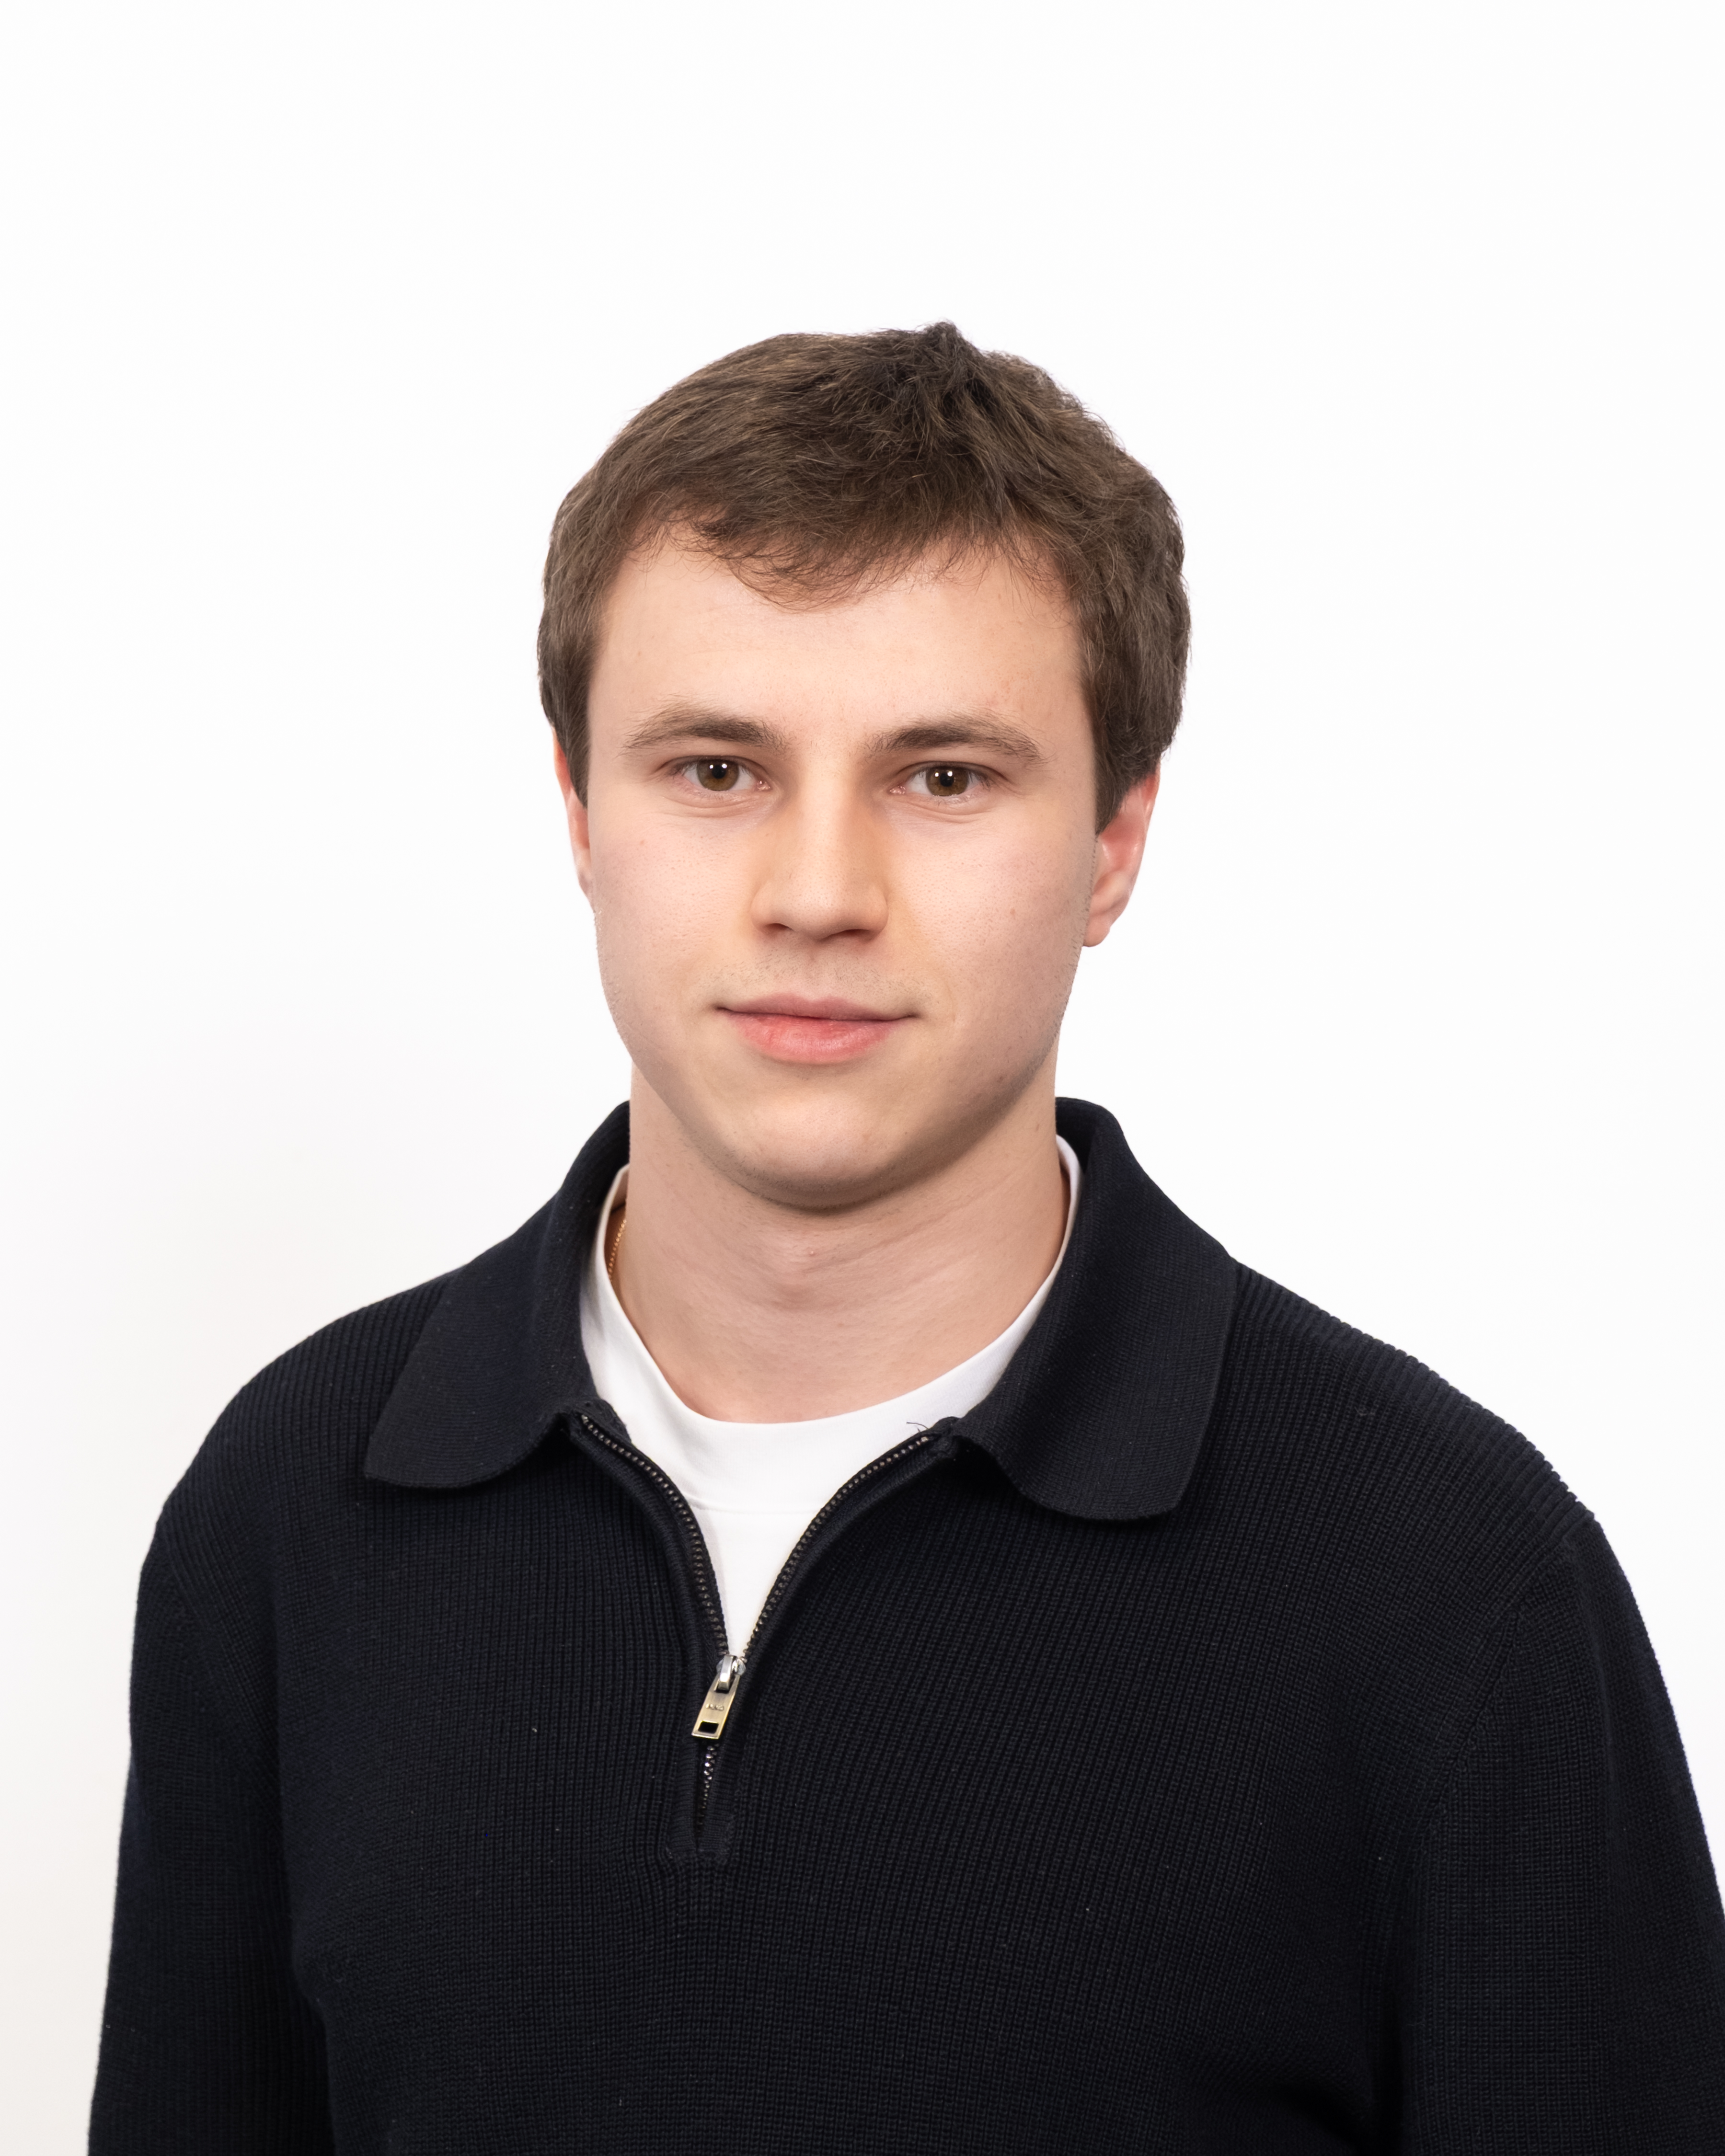
\includegraphics[width=1.6cm, keepaspectratio]{../../resources/img/photo.png}};
%     \end{tikzpicture}
% \end{minipage}

% %----------------------------------------------------------------------------------------
% % PROFILE
% %----------------------------------------------------------------------------------------
% \vspace{-15pt}

% \cvtextnotab{
%     \fontsize{9.5pt}{11pt}\selectfont
%     Ingénieur en informatique spécialisé en \textbf{Data Engineering, Machine Learning et calcul scientifique},
%     avec 3 ans d'expérience en alternance chez \textbf{Société Générale Assurances}.
%     Solide formation en \textbf{mathématiques appliquées, probabilités, statistiques, optimisation et algorithmique},
%     avec un intérêt particulier pour le \textbf{Quantitative Development, Quantitative Research et les marchés financiers}.
% }
%---------------------------------------------------------------------------------------
% HEADER
%---------------------------------------------------------------------------------------
\pdfbookmark[1]{Contact}{contact}

\noindent
\begin{minipage}[t]{0.865\textwidth}
    \vspace{-4pt}

    % NAME + TARGET POSITION
    \begin{center}
        {\textbf{\fontsize{15pt}{10pt}\selectfont Dmytro Palahin}}\\[-1pt]
        {\textbf{\fontsize{9.5pt}{10pt}\selectfont Quantitative Researcher / Quantitative Engineer}}
    \end{center}

    \vspace{-19pt}

    % CONTACTS
    \begin{center}
        {\fontsize{8.7pt}{10pt}\selectfont
            \locationIcon[black]\hspace{2pt}Paris, France
            \hspace{10pt}
            \href{tel:+33787325878}{\phoneIcon[black]\hspace{2pt}+33 7 87 32 58 78}
            \hspace{10pt}
            \emailLink[black]{dmytro.palahin@gmail.com}
            \hspace{10pt}
            \linkedinIcon[black]\hspace{2pt}\href{https://www.linkedin.com/in/dmytro-palahin/}{Dmytro Palahin}
            \hspace{10pt}
            \githubIcon[black]\hspace{2pt}\href{https://github.com/DmytroPalahin}{DmytroPalahin}
        }
    \end{center}

    \vspace{-6pt}

    % PROFIL
    {\fontsize{8.7pt}{9.6pt}\selectfont
        Élève-ingénieur en informatique en dernière année avec \textbf{3 ans d'expérience en Data Engineering,
            Machine Learning et MLOps} chez \textbf{Société Générale Assurances}.
        Solide formation en \textbf{mathématiques appliquées, probabilités, statistiques,
            optimisation et algorithmique}, complétée par une expérience en
        \textbf{calcul scientifique et traitement de données à grande échelle}.
        Intéressé par la \textbf{finance quantitative, le trading systématique et les stratégies basées sur les données},
        avec un intérêt particulier pour la \textbf{recherche quantitative, la modélisation statistique et l'analyse des données de marché}.
    }

\end{minipage}
\hfill
\begin{minipage}[t]{0.115\textwidth}
    \vspace{1pt}
    \centering
    \begin{tikzpicture}
        \clip (0,0) circle (0.88cm);
        \node at (0,0) {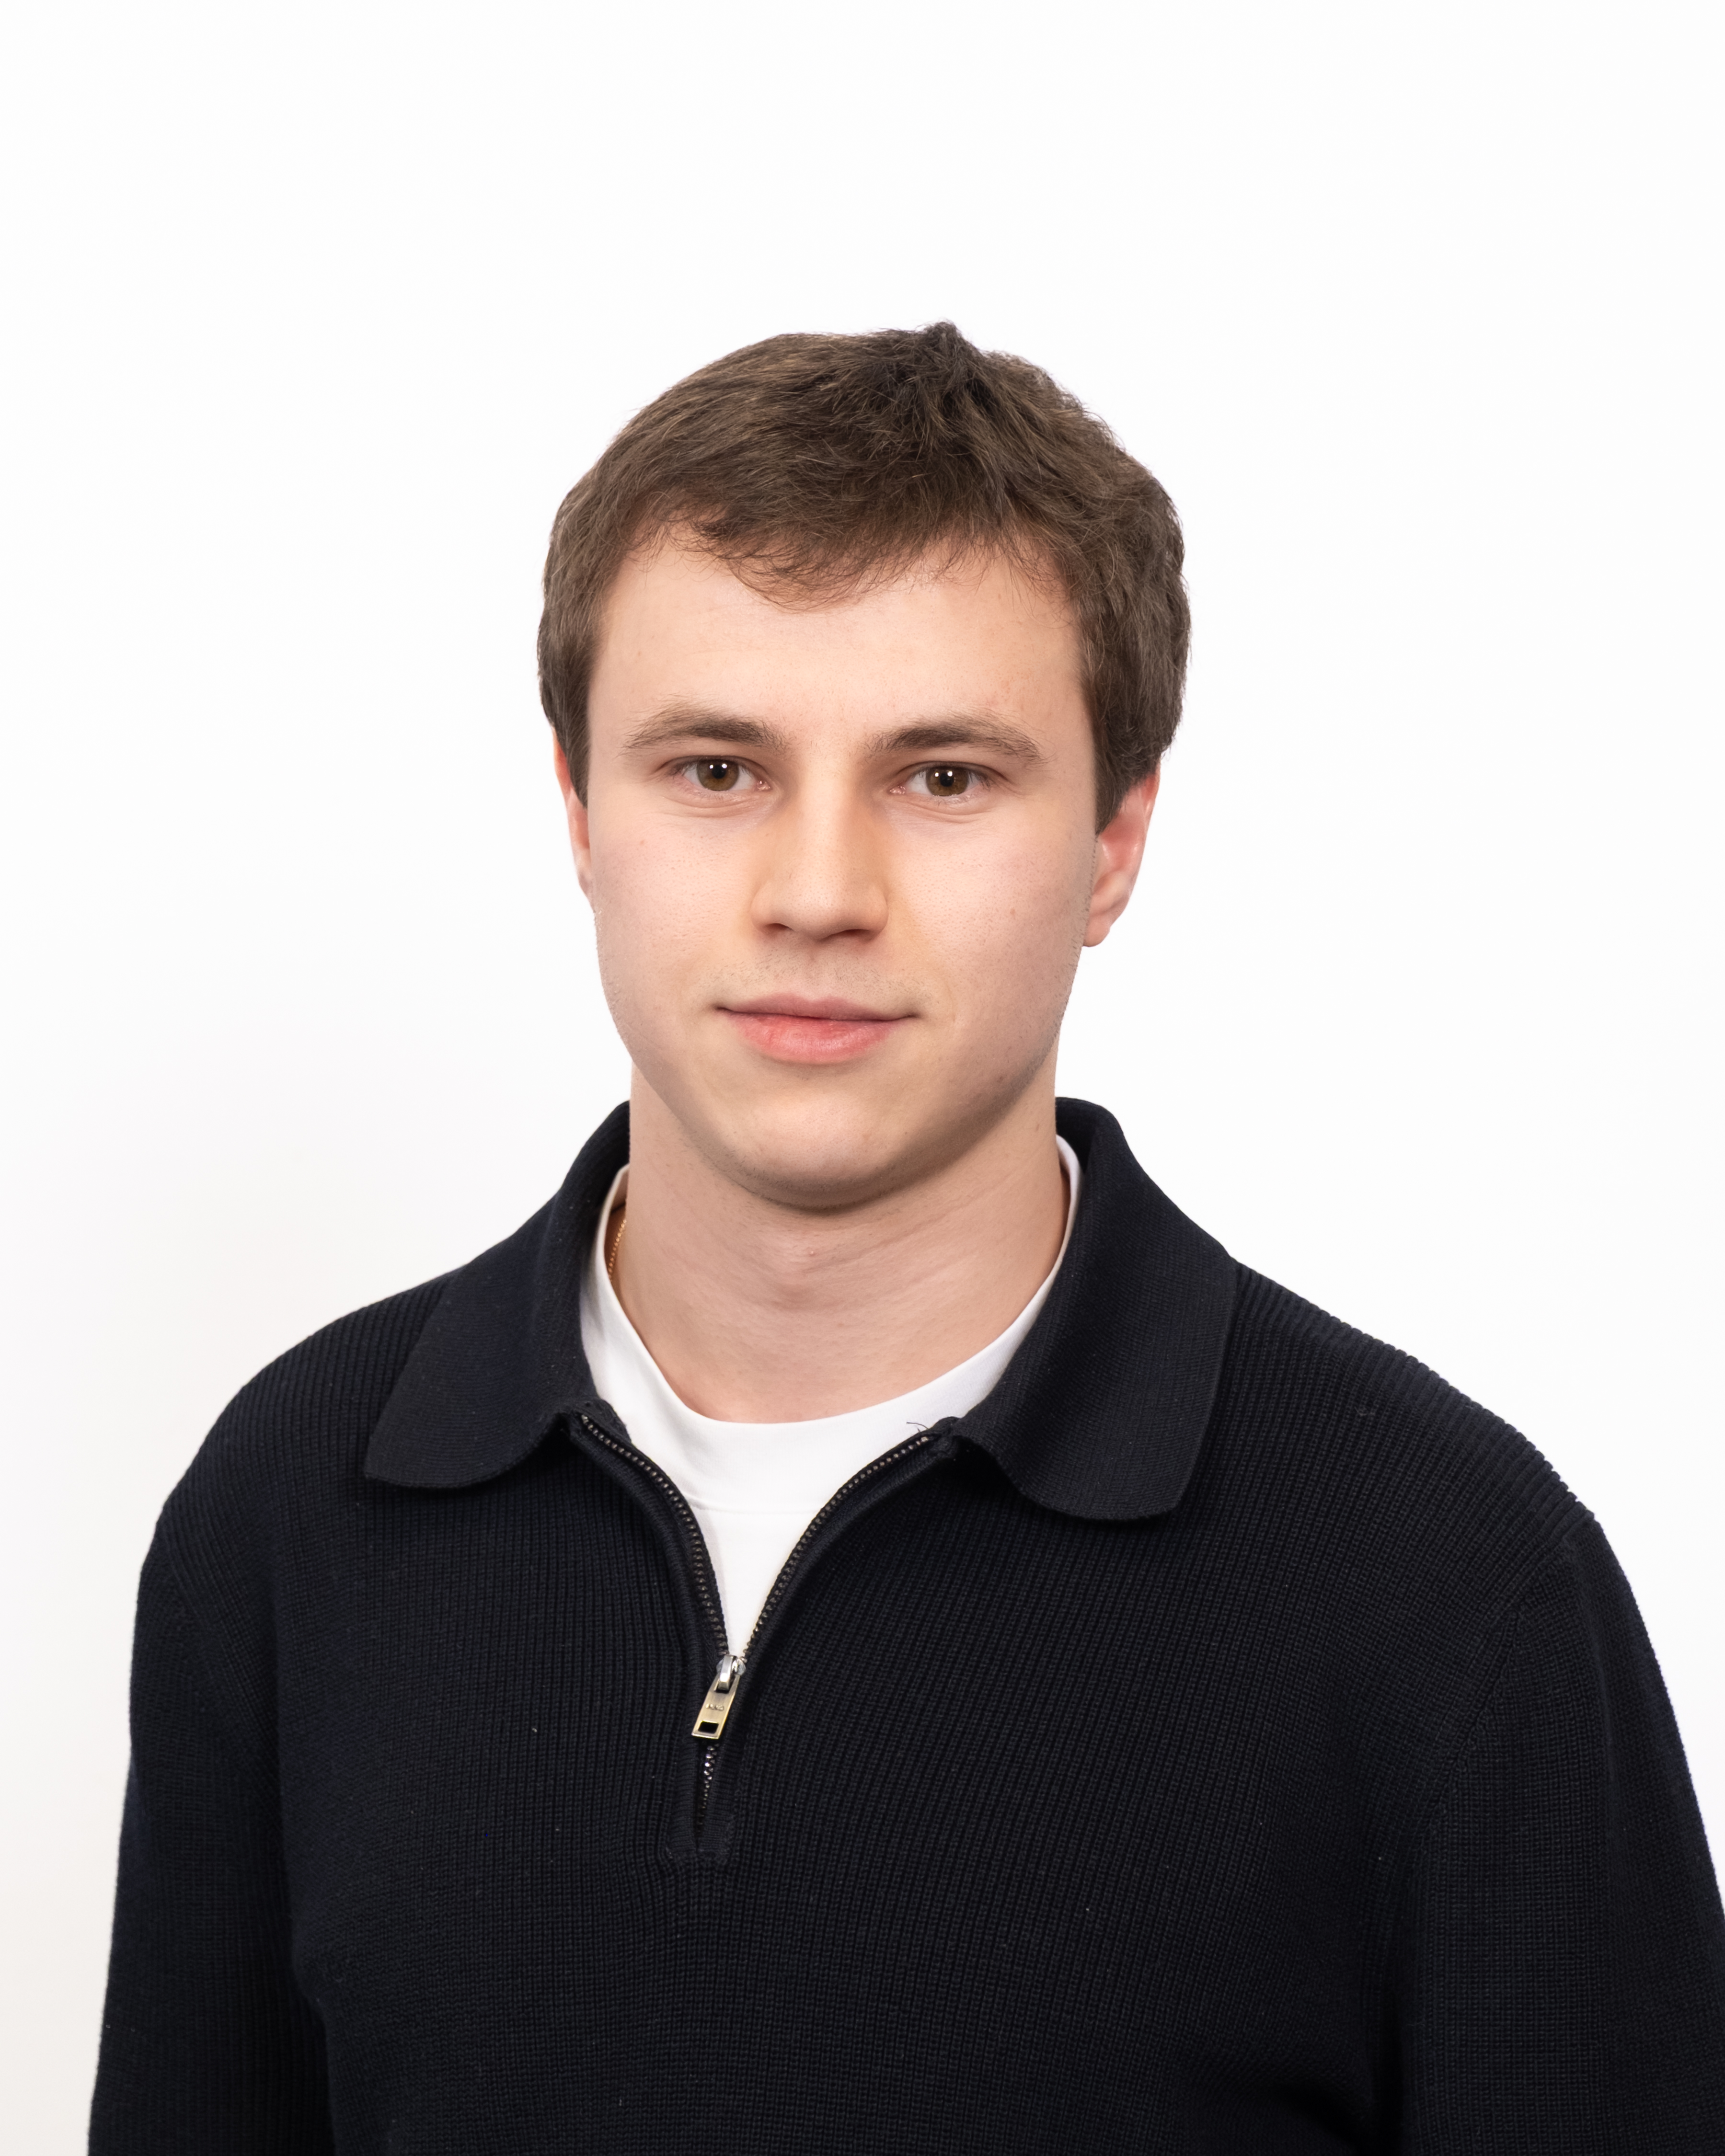
\includegraphics[width=1.55cm, keepaspectratio]{../../resources/img/photo.png}};
    \end{tikzpicture}
\end{minipage}

\vspace{2pt}

%----------------------------------------------------------------------------------------
% PROFESSIONAL EXPERIENCE
%----------------------------------------------------------------------------------------
\vspace{1pt}
\pdfbookmark[1]{Expérience}{work_exp}
\cvsection{\workIcon[black]\hspace{4pt}EXPÉRIENCE PROFESSIONNELLE}

\vspace{-4pt}
\pdfbookmark[2]{Société Générale}{sg}
\cvevent{Data Engineer / MLOps (Alternance) --- Société Générale Assurances}{\fontsize{11pt}{11pt}\selectfont 09/2023\hspace{5pt}--\hspace{5pt}Aujourd'hui}
\cvsubevent{La Défense, France}{}

\vspace{-5pt}
\begin{itemize}[leftmargin=0.5cm, label=\textbullet, itemsep=0.05em]
    \item Analyse de \textbf{1 an de données opérationnelles} du \textbf{Callbot Zaion}
          avec Python afin d'identifier les principales sources d'erreurs,
          d'évaluer la performance du système et de formuler \textbf{3 recommandations d'amélioration}
          \begin{itemize}[leftmargin=0.25cm,label=\textendash,itemsep=0em,topsep=0.1em]
              \item \textit{\fontsize{10pt}{9pt}\selectfont Python · Pandas · NumPy · Jupyter Notebook · Matplotlib · Plotly}
          \end{itemize}

    \item Conception d'un \textbf{système automatisé de migration SAS Guide vers Python},
          intégrant des traitements de données avec \textbf{Polars et DuckDB},
          du prompt engineering et une \textbf{validation automatisée par tests à 2 niveaux}
          \begin{itemize}[leftmargin=0.25cm,label=\textendash,itemsep=0em,topsep=0.1em]
              \item \textit{\fontsize{10pt}{9pt}\selectfont Python · Polars · DuckDB · GitHub Copilot · AWS S3}
          \end{itemize}

    \item Conception et automatisation d'un \textbf{pipeline de traitement et migration de données}
          permettant le transfert de \textbf{500\raisebox{0.20ex}{\small +} GB de datasets SAS Guide vers AWS S3}
          et leur mise à disposition pour les équipes Data
          \begin{itemize}[leftmargin=0.25cm,label=\textendash,itemsep=0em,topsep=0.1em]
              \item \textit{\fontsize{10pt}{9pt}\selectfont Python · AWS S3 · fsspec · smbfs · Linux · Bash}
          \end{itemize}

          % \item Développement et déploiement de \textbf{3 extensions VS-Code} afin de simplifier
          %       l'utilisation d'outils internes sur la \textbf{plateforme Data} et d'améliorer
          %       l'efficacité des workflows pour \textbf{30\raisebox{0.20ex}{\small +} utilisateurs
          %           (Data Scientists \& Data Analysts)}
          %       \begin{itemize}[leftmargin=0.25cm,label=\textendash,itemsep=0em,topsep=0.2em]
          %           \item \textit{\fontsize{10pt}{9pt}\selectfont TypeScript · Python · JSON · Bash · Linux · Git · VS-Code}
          %       \end{itemize}

          % \item Improvement of an \textbf{internal access management tool} to simplify the
          %       administration of \textbf{user rights} for \textbf{30\raisebox{0.20ex}{\small
          %               +} users} in Data teams
          %       \begin{itemize}[leftmargin=0.25cm,label=\textendash,itemsep=0em,topsep=0.2em]
          %           \item \textit{\fontsize{10pt}{9pt}\selectfont Python · JavaScript · API · Git}
          %       \end{itemize}

          % \item Maintenance et mise à jour de \textbf{35\raisebox{0.20ex}{\small +} extensions
          %           internes} ainsi que des \textbf{versions de code-server} afin de garantir la
          %       \textbf{stabilité et la compatibilité de l'environnement de développement} utilisé par
          %       \textbf{40\raisebox{0.20ex}{\small +} utilisateurs} des équipes Data
          %       \begin{itemize}[leftmargin=0.25cm,label=\textendash,itemsep=0em,topsep=0.2em]
          %           \item \textit{\fontsize{10pt}{9pt}\selectfont Linux · Bash · VS Code · code-server · Git}
          %       \end{itemize}

          % \item Analysis and comparison of \textbf{two data tables (SAS Guide vs DataLake S3)} on
          %       \textbf{several thousand rows} via \textbf{matching methods and gap analysis},
          %       enabling the identification of \textbf{data inconsistencies and discrepancies}
          %       in a migration project
          %       \begin{itemize}[leftmargin=0.25cm,label=\textendash,itemsep=0em,topsep=0.2em]
          %           \item \textit{\fontsize{10pt}{9pt}\selectfont Python · Pandas · SAS Guide · AWS S3 · Jupyter Notebook · Git}
          %       \end{itemize}
\end{itemize}

% \pdfbookmark[2]{IT Company SPD}{spd}
% \vspace{-5pt}
% \cvevent{\textbf{Training at IT Company SPD Ukraine} --- Machine Learning / Deep Learning}{\fontsize{11pt}{11pt}\selectfont 2022}
% \cvsubevent{}{Cherkasy, Ukraine}
% \vspace{-18pt}
% \begin{itemize}[leftmargin=0.75cm,label=\textendash,itemsep=0em,topsep=0.2em]
%     \item \textit{\fontsize{10pt}{9pt}\selectfont Scikit-Learn · Pandas · NumPy · Matplotlib · Seaborn · TensorFlow · XGBoost}
% \end{itemize}

%----------------------------------------------------------------------------------------
% IT PROJECTS
%----------------------------------------------------------------------------------------
\vspace{-4pt}
\pdfbookmark[1]{Projets}{projects}
\vspace{-4pt}
\cvsection{\itProjectIcon[black]\hspace{4pt}PROJETS TECHNIQUES \& SCIENTIFIQUES}

\vspace{-7pt}
\begin{itemize}[leftmargin=0.5cm, label=\textbullet, itemsep=0.12em]
    \pdfbookmark[2]{Placement de centres logistiques}{logistics}
    \item \href{https://github.com/DmytroPalahin/logistics-center-placement}
          {\textbf{Optimisation combinatoire de centres logistiques}} |
          \textit{Python, Julia, CPLEX, MILP} \hfill \textbf{2025}

          Modélisation et résolution d'un problème de placement par
          \textbf{programmation linéaire en nombres entiers}, CPLEX et méthodes heuristiques

          \pdfbookmark[2]{Article}{article}
    \item \href{https://www.researchsquare.com/article/rs-2203260/v1}
          {\textbf{Publication scientifique --- Algorithmes mathématiques}} \hfill \textbf{2021}

          Développement d'une méthode mathématique de filtrage du bruit impulsionnel dans les images vidéo,
          publiée dans \textit{Informatics and Mathematical Methods in Simulation}, Vol. 11, No. 4

          \pdfbookmark[2]{Détection d'anomalies}{anomaly_detection}
    \item \href{https://github.com/DmytroPalahin/Anomaly_Detection}
          {\textbf{Détection d'anomalies}} | \textit{Python, Machine Learning} \hfill \textbf{2021}

          Étude de méthodes de détection d'anomalies et d'étiquetage partiel de données

          \pdfbookmark[2]{Problème du voyageur}{salesman}
    \item \href{https://github.com/DmytroPalahin/Probleme_du_Voyageur_de_Commerce}
          {\textbf{Problème du voyageur de commerce}} |
          \textit{C, Optimisation combinatoire, Métaheuristiques} \hfill \textbf{2023}

          Implémentation en C d'un algorithme d'optimisation par \textbf{colonies de fourmis}

          \pdfbookmark[2]{Détection de phishing par email}{phishing}
    \item \href{https://github.com/DmytroPalahin/phishing-email-detection}
          {\textbf{Détection de phishing par Machine Learning}} |
          \textit{Python, Machine Learning, NLP} \hfill \textbf{2026}

          Classification de \textbf{76\,677 emails} issus de 5 datasets réels via
          TF-IDF, LightGBM, Naive Bayes et LSTM
\end{itemize}

% Future Quant projects — keep commented until they are actually completed:
% \begin{itemize}[leftmargin=0.5cm, label=\textbullet, itemsep=0.12em]
%     \item \textbf{Option Pricing \& Monte Carlo} | \textit{Python/C++, NumPy, Black--Scholes, Monte Carlo}
%     \item \textbf{Quantitative Strategy Research \& Backtesting} | \textit{Python, Time Series, Risk Metrics, Walk-Forward Analysis}
% \end{itemize}

%----------------------------------------------------------------------------------------
% EDUCATION
%----------------------------------------------------------------------------------------
\vspace{-5pt}
\pdfbookmark[1]{Formation}{education}
\cvsection{\educationIcon[black]\hspace{4pt}FORMATION}

\vspace{-3pt}
\pdfbookmark[2]{Sup Galilée}{sup_galilee}
\cvevent{\href{https://www.sup-galilee.univ-paris13.fr/}{École d'ingénieurs Sup Galilée} --- Diplôme d'ingénieur en Informatique \textit{(en cours)}}{\fontsize{11pt}{11pt}\selectfont 2023\hspace{5pt}--\hspace{5pt}2026}
% \cvsubevent{}{Villetaneuse, France}

\vspace{-3pt}
\cvtextnotab{
    \textbf{Cours\!:}
    Probabilités et Statistiques, Optimisation linéaire et combinatoire,
    Méthodes numériques, Data Mining, Programmation pour l'IA,
    Algorithmique et Complexité, Algorithmique des graphes,
    C/C++, Algorithmes parallèles et distribués,
    Bases de données avancées, Cloud Computing
}
% 1. Mathématiques
% 1.1 Algèbre linéaire  
% Espaces vectoriels  
% Matrices  
% Déterminants  
% Valeurs propres  
% Diagonalisation  
% Formes bilinéaires  
% Formes quadratiques  

% 1.2 Analyse mathématique   
% Limites  
% Continuité  
% Dérivabilité  
% Développements de Taylor  
% Matrice hessienne  
% Matrice jacobienne  
% Dérivées partielles  
% Intégrales doubles et triples  
% Changement de variables  
% Équations différentielles  

% 1.3 Probabilités  
% Probabilités  
% Probabilités conditionnelles  
% Variables aléatoires  
% Loi gaussienne  
% Loi exponentielle  
% Lois continues  

% 1.4 Statistiques  
% Tu avais notamment :  
% Probabilités et Statistiques  
% Data Mining  

% 1.5 Optimisation  
% Optimisation linéaire et optimisation combinatoire

% 2. Informatique
% Algorithmes  
% Algorithmes sur les graphes  
% Complexité  
% C  
% C++  
% Java  
% Programmation fonctionnelle  
% Logique  
% Bases de données  
% Bases de données avancées  
% Cloud  
% Algorithmes distribués  
% Algorithmes parallèles  
% Cryptographie  
% Programmation en intelligence artificielle
% Cybersecurity
% UML
% Analysis / Algebra
% Cryptography
% Complexity
% Compilation and language theory
% Functional programming
% Logic programming
% System administration
% Network administration
% Computer architecture
% Numerical methods
% Semantic web
% Logic
% Operating systems
% C/C++
% Web (TS/JS)

\vspace{-10pt}
\noindent{\textcolor{middle_light_gray}{\rule{\mpwidth}{0.2pt}}}
\vspace{-15pt}

\pdfbookmark[2]{Classe préparatoire}{prepa}
\cvevent{\href{https://www.univ-spn.fr}{Université Sorbonne Paris Nord} --- \href{https://www.sup-galilee.univ-paris13.fr/index.php/formation/cp2i/}{Classe préparatoire à \textbf{Sup Galilée}}}{\fontsize{11pt}{11pt}\selectfont 2021\hspace{5pt}--\hspace{5pt}2023}
% \cvsubevent{}{Villetaneuse, France}

\vspace{-10pt}
\cvtextnotab{
    \textbf{Cours\!:}
    Algèbre linéaire (espaces vectoriels, matrices, valeurs propres, diagonalisation),
    Analyse multivariable (dérivées partielles, Jacobienne, Hessienne, séries de Taylor),
    Probabilités (variables aléatoires, probabilités conditionnelles, lois usuelles),
    équations différentielles et calcul numérique
}

% \vspace{-5pt}
% \noindent{\textcolor{middle_light_gray}{\rule{\mpwidth}{0.2pt}}}
% \vspace{-10pt}

% \pdfbookmark[2]{High School}{high_school}
% \cvevent{Phymly High School --- Specialization in Mathematics, Physics and Computer Science}{\fontsize{11pt}{11pt}\selectfont 2016\hspace{5pt}--\hspace{5pt}2021}
% \cvsubevent{}{Cherkasy, Ukraine}

%----------------------------------------------------------------------------------------
% CERTIFICATIONS & SKILLS
%----------------------------------------------------------------------------------------
\vspace{-8pt}
\pdfbookmark[1]{Certifications et Compétences}{certifications_competences}
\cvsection{\certificateIcon[black]\hspace{4pt}CERTIFICATIONS \& COMPÉTENCES}

\vspace{-4pt}
\begin{itemize}[leftmargin=0.5cm, label=\textbullet, itemsep=0.12em]

    \item \textbf{Programmation \& Calcul scientifique\!:}
          C/C++, Python, Julia, Matlab, SQL, SAS Guide, Java, Haskell ·
          NumPy, Pandas, Polars, DuckDB ·
          Git, Linux, Jupyter

    \item \textbf{Algorithmique \& Informatique\!:}
          Structures de données, complexité algorithmique,
          algorithmique des graphes, programmation parallèle et distribuée

    \item \textbf{Mathématiques appliquées\!:}
          Algèbre linéaire, probabilités et statistiques,
          méthodes numériques, optimisation,
          simulation de Monte Carlo et modélisation stochastique

    \item \textbf{Machine Learning\!:}
          Scikit-Learn, LightGBM, XGBoost, TensorFlow/Keras ·
          Data Mining, classification, détection d'anomalies

    \item \textbf{Marchés financiers \& Données de marché\!:}
          Forex, actions, futures ·
          Microstructure, carnet d'ordres (L2/L3), market data,
          liquidité, types d'ordres, exécution, VWAP ·
          Rapports COT (Commitments of Traders), gestion du risque

          % À ajouter uniquement après pratique réelle :
          % C++17/20, STL, multithreading, SciPy, FIX Protocol, QuantLib,
          % séries temporelles, Order Book L2/L3, Interactive Brokers API, Binance API

    \item \textbf{Udemy\!:}
          \href{https://www.udemy.com/certificate/UC-51319000-ccb8-4c9c-9320-6cd9860e601c/}
          {\textit{Python for Data Science and Machine Learning Bootcamp}}
          --- Jose Portilla / Pierian Training
\end{itemize}

%----------------------------------------------------------------------------------------
% AWARDS & PARTICIPATIONS
%----------------------------------------------------------------------------------------
\vspace{-3pt}
\pdfbookmark[1]{Participations}{participations}
\cvsection{\awardIcon[black]\hspace{4pt}PRIX \& PARTICIPATIONS}

\vspace{-6pt}
\begin{itemize}[leftmargin=0.35cm, label=\textbullet, itemsep=0.15em]
    \item \textbf{\href{https://www.fondationbesse.com/}{Lauréat de la Fondation Georges Besse}}
    \item \textbf{Eco\hspace{3pt}--\hspace{3pt}Techno Ukraine ISEF} --- 1\textsuperscript{ère} place en Informatique \& \textbf{Service Internet Intelligence Collective} --- 1\textsuperscript{ère} place en Ukraine
\end{itemize}

%----------------------------------------------------------------------------------------
% LANGUAGES & INTERESTS
%----------------------------------------------------------------------------------------
\vspace{-5pt}
\pdfbookmark[1]{Langues et centres d'intérêt}{languages_interests}
\cvsection{\speechBubbleIcon[black]\hspace{4pt}LANGUES \& CENTRES D'INTÉRÊT}

\vspace{-3pt}
\cvtextnotab{\textbf{Français\!:} Courant \hspace{12pt} \textbf{Anglais\!:} Courant \hspace{12pt} \textbf{Ukrainien\!:} Natif \hspace{20pt} \textbf{Russe\!:} Bilingue}

\vspace{-8pt}
\cvtextnotab{
    \tradingIcon[black]\hspace{2pt}Marchés financiers / Trading \hspace{12pt}
    % \cryptoIcon[black]\hspace{2pt}Crypto \hspace{12pt}
    \chessIcon[black]\hspace{2pt}Échecs \hspace{12pt}
    \skiIcon[black]\hspace{2pt}Ski \hspace{12pt}
    \tennisIcon[black]\hspace{2pt}Tennis \hspace{12pt}
    \swimmingIcon[black]\hspace{2pt}Natation \hspace{12pt}
    % \mountainsIcon[black]\hspace{2pt}Hiking
    \flagIcon[black]\hspace{2pt}Karting | Formula 1
}

\end{document}

/*
latexmk -pdf cv-dmytro-palahin-fr-q.tex
latexmk -pdf -auxdir=/tmp/latex-build -outdir=. cv-dmytro-palahin-fr-q.tex
pdftoppm -png -r 600 cv-dmytro-palahin-fr-q.pdf ./img/cv-dmytro-palahin-fr-q
*/
